\documentclass[a4paper,10pt]{article}
\usepackage[utf8]{inputenc}
\usepackage{graphicx}
\usepackage{subcaption}
\usepackage{parskip}
\usepackage{amsmath}
\usepackage{listings}
\usepackage{color}
\usepackage{listings}

\definecolor{red}{rgb}{1,0,0}
\definecolor{green}{rgb}{0,1,0}
\definecolor{codegreen}{rgb}{0,0.6,0}
\definecolor{codegray}{rgb}{0.5,0.5,0.5}
\definecolor{codepurple}{rgb}{0.58,0,0.82}
\definecolor{backcolour}{rgb}{0.95,0.95,0.92}

\lstdefinestyle{mystyle}{
    backgroundcolor=\color{backcolour},   
    commentstyle=\color{blue},
    numberstyle=\tiny\color{codepurple},
    stringstyle=\color{codegreen},
    basicstyle=\footnotesize,
    breakatwhitespace=false,         
    breaklines=true,                 
    captionpos=b,                    
    keepspaces=true,                 
    numbers=left,                    
    numbersep=5pt,                  
    showspaces=false,                
    showstringspaces=false,
    showtabs=false,                  
    tabsize=2
}
 
\lstset{style=mystyle,language = Python}

%opening
\title{Swiggity Swooty, Project 2}
\author{Joe}

\begin{document}

\maketitle

\section{Pores}
To begin with, we've created an fcc lattice of 20$\times$20$\times$20 fcc unit blocks, concluding in a 32000 particle crystal. We now generate 20 spheres in which particles will not move.
The pores' centers are randomly distributed somewhere INSIDE the block. This allows large parts of the pores to exist outside of the block and for fixed spheres to overlap (see fig \ref{fig1}).


The porosity is the relationship between the pore space and the original crystal. Thinking creatively, this is the same as the relation between the deleted atoms to the original ones:
13954/32000 which is equivalent to $43.6\%$.

Since our pores overlap with the boundaries and themselves, we are still left with particles. If the pores had been non-overlapping, there would be no moving particles left.
\begin{figure}\centering
 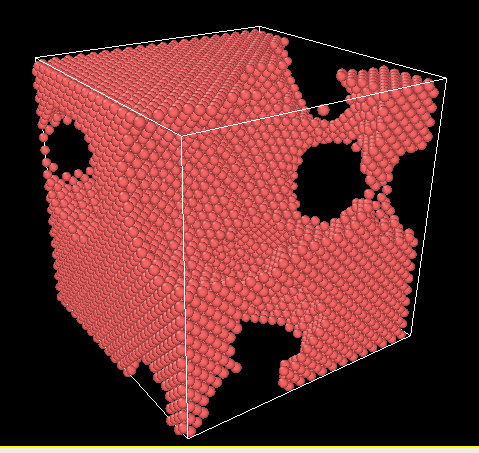
\includegraphics[width=0.55\linewidth]{pore}
 \caption{20 spherical pores (voids) are generated inside a block of orginally 32000 particles.}
 \label{fig1}
\end{figure}



\end{document}
